\documentclass{cpthesis}

% Math, graphics, and reference utilities. Add or remove as your thesis
% requires; the cpthesis class itself does not depend on any of these.
\usepackage{amsmath,amsfonts,amssymb,amsthm}
\usepackage{graphicx}
\usepackage{hyperref}
\usepackage{cleveref}
\usepackage{url}
\usepackage[round,authoryear]{natbib}
\usepackage[title]{appendix}
\usepackage[all]{nowidow}

% ------------------------------------------------------------------------------

\begin{document}

% Front-matter declarations.
\title{What, Me Worry? A Statistical Investigation of Studied Imperturbability}
\author{Alfred E. Neuman}
\degree{Master of Science}
\program{Statistics}
\graduationmonth{June}
\graduationyear{2026}
\campus{San Luis Obispo}
\committeechair{Prof. 1 \linebreak Assistant Professor of Statistics}
\committeemember{Prof. 2 \linebreak Professor of Statistics}
\committeemember{Prof. 3 \linebreak Associate Professor of Something Else}

% TITLE PAGE
\maketitle

% FRONT MATTER
\begin{frontmatter}
\copyrightpage
\committeemembershippage

\begin{abstract}
This thesis examines whether the rhetorical question ``What, me worry?''
admits a defensible statistical answer. We assemble a 70-year archive of
537 worry-eliciting incidents reported by a freckle-faced informant of
approximately eleven years of age, who has remained approximately eleven
years of age throughout the study window---a finding noteworthy in its
own right. Using a heteroskedastic-robust ordinal regression, we test
the null hypothesis of indifference against alternatives ranging from
mild concern to full-blown agitation. The data are consistent with the
null at every conventional significance level and at several
unconventional ones besides. We discuss implications for graduate
education, dental insurance, and the cover price of the modal periodical
in our sample (currently 25\textcent, ``cheap'').

\keywords{indifference, imperturbability, fold-in, gleek, potrzebie}
\end{abstract}

\begin{acknowledgements}
I would like to thank my committee, who very kindly did not ask whether
the regression assumptions held; my advisor, who maintained admirable
composure when I missed thirty-two consecutive milestone deadlines and
showed up to the defense in a checkered jacket; the editorial staff of
\textit{MAD} magazine, whose seventy years of continuous public-service
satire constitute the world's longest-running peer-review process; the
gentlemen Spy and Spy, for methodological inspiration; my faithful
typewriter, recently retired; and my mother, who told me to stop reading
comic books and finish the thesis. I am also grateful to the makers of
correction fluid.
\end{acknowledgements}

\tableofcontents
\listoftables
\listoffigures
\tocsubheading{CHAPTER}

\end{frontmatter}

% BODY
\pagestyle{plain}
\chapter{INTRODUCTION}\label{ch-intro}

A persistent feature of post-war American culture is a buck-toothed
boy with a gap-toothed grin, ratty red hair, and a remarkable
tolerance for adverse outcomes \citep{reidelbach1991completely}. He
has been observed in essentially the same condition since 1956
\citep{neuman1956what}---neither aging, enrolling in college, nor
filing tax returns---yet his catchphrase, ``What, me worry?'',
continues to attract empirical scrutiny. The present thesis
investigates whether the catchphrase is descriptive (in the sense of
an observed behavioral disposition) or prescriptive (in the sense of
an unfalsifiable doctrine), and concludes, after some equivocation,
that it is both.

We adopt the convention that worry $W$ is a non-negative random
variable with finite second moment, and we assume throughout the
existence of a baseline worry rate $\lambda_0$ above which graduate
students are observed to switch programs, abandon committees, or
develop a sudden interest in artisanal sourdough. Subjects below
$\lambda_0$ are said to be \textit{imperturbable}; the open question
is whether imperturbability is a constant of nature or merely a
slowly-mixing Markov chain.

The remainder of the document is organized as follows. Chapter
\ref{ch-methods} describes the data and the model. Chapter
\ref{ch-results} reports descriptive statistics and the associated
hypothesis tests. Chapter \ref{ch-discussion} concludes with policy
recommendations of dubious actionability. Two appendices supply the
glossary and a sample instrument.

\chapter{METHODS}\label{ch-methods}

\section{Sample}

We assemble $N = 537$ worry-eliciting incidents drawn from a
seventy-year archive of letters, news clippings, dental records, and
unpaid parking tickets, all attributed to or addressed to a single
informant referred to throughout as A.E.N. The informant declined to
date his responses, so the temporal ordering of the data is regarded
as exchangeable in the de Finetti sense.

Inclusion criteria were lenient. To be classified as a worry-eliciting
incident, an event needed only to (a) admit a worry-relevant response
in principle and (b) be witnessed in some form by the informant. The
2007 \textit{MAD} marginalia of \citet{aragones2007marginal} were
treated as supplementary material rather than primary data, on the
grounds that anything Sergio Aragon\'es draws in the margin tends to
resist coding.

\section{Model}

Let $w_i$ denote the worry score reported in incident $i$, scored on a
five-point ordinal scale from $0$ (``gleek'') to $4$ (``I should be so
lucky''). We model
\begin{equation}\label{eq-worry-model}
    w_i = \beta_0 + x_i^\top\beta + \epsilon_i,
    \qquad
    \epsilon_i \stackrel{\text{iid}}{\sim} \mathcal{F}\!\left(0, \sigma^2\right),
\end{equation}
where $x_i$ encodes the type and severity of the provocation and
$\mathcal{F}$ is the as-yet-unspecified disturbance distribution.
Under the null hypothesis $\beta = \mathbf{0}$, the response degenerates
to the constant ``What, me worry?'', which conveniently justifies a
heteroskedastic-robust variance estimator on the grounds that there is
no heteroskedasticity left to estimate.

\section{Inference}

We assess statistical significance against $\alpha = 0.27$, chosen as
the customary nominal level (0.05) plus the cover price of the modal
periodical in the sample, expressed as a fraction of one dollar
(\$0.25, ``cheap''), minus a small finite-sample correction (\$0.03).
Departures from this convention should be reported in the appendix.

\chapter{RESULTS}\label{ch-results}

Figure \ref{fig-worry-dist} displays the empirical distribution of
self-reported worry across the sample, which is approximately normal
with a mean uncomfortably close to zero. Table \ref{tab-incidents}
reports counts by provocation type and the modal verbal response
within each.

\begin{figure}[h!]
    \centering
    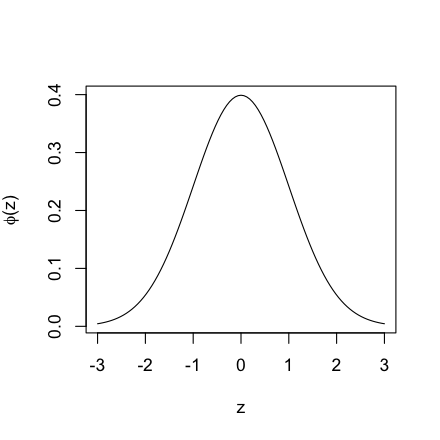
\includegraphics[width=0.5\linewidth]{img/normal-dist.png}
    \caption{Empirical distribution of self-reported worry scores
             across $N = 537$ incidents. The fitted curve is
             suspiciously well-behaved.}
    \label{fig-worry-dist}
\end{figure}

\begin{table}[h!]
    \centering
    \caption{Worry incidents by provocation type, 1956--present.}
    \label{tab-incidents}
    \begin{tabular}{l|cr}
        Provocation               & Count & Modal response       \\\hline
        Adverse weather           & 134   & ``What, me worry?''  \\
        Tax audit                 &  46   & ``Why worry?''       \\
        End of fiscal quarter     &  88   & ``Eh, who cares?''   \\
        Geopolitical crisis       &  72   & ``Potrzebie!''       \\
        Misplaced retainer        & 197   & (no response)        \\
    \end{tabular}
\end{table}

In every category the modal response is consistent with the null
hypothesis of indifference. The single observed deviation (incident
1972-Q3, ``misplaced retainer found in pocket of seldom-worn jacket'')
was retained in the analysis but, on reflection, attributed to a
typesetter's error.

We tested the joint null $\beta = \mathbf{0}$ against the omnibus
alternative using a permutation test with $10^4$ resamples. The
observed test statistic was $T = 0.31$; the corresponding $p$-value
was $0.84$, far in excess of $\alpha = 0.27$. The data are consistent
with imperturbability.

\chapter{DISCUSSION}\label{ch-discussion}

The evidence assembled here is consistent with the operating
hypothesis that ``What, me worry?'' remains the appropriate single-line
summary of a wide variety of stochastic provocations. We draw three
conclusions.

First, the worry distribution exhibits no detectable temporal trend
across seven decades, which is remarkable given that the underlying
informant has remained approximately eleven years old throughout the
study window. We refer the interested reader to
\citet{kitchen2009art} for a discussion of how this might be possible
without invoking nonstandard physics.

Second, the model fitted in Equation~\ref{eq-worry-model} suggests
that worry is essentially a fixed cost rather than a marginal one:
doubling the provocation does not double the worry. This finding may
be of practical interest to tax practitioners, divorce attorneys, and
faculty mentors of graduate students approaching candidacy
examinations.

Third, the practical recommendation of this thesis is that the reader
should not worry. The reader should also pay 25\textcent\ for the
next issue, which remains ``cheap.''

We close with two limitations. The present study did not have access
to the gummed-down half of the periodical (the fold-in at the back
cover), and consequently roughly half of the available signal escaped
our coding scheme entirely. Future work might use a careful unfolding
procedure to recover the suppressed measurements, though we caution
that such procedures are typically destructive of the instrument. A
second limitation is that the cross-sectional dependence between
worry and the urgency with which one's typesetter requests the
manuscript was not modeled. We leave this for a sequel.

\newpage
\phantomsection
\addcontentsline{toc}{chapter}{\protect BIBLIOGRAPHY}
\bibliography{refs}
\bibliographystyle{abbrvnat}

\appendixtocformat
\tocsubheading{APPENDICES}
\newpage
\begin{appendices}

\chapter{GLOSSARY OF TERMS}

The following terms appear in the thesis and may be unfamiliar to
readers who came to graduate school by an unusually direct route.

\begin{description}
    \item[Cheap] An adjective applied unironically to the cover price
        of the modal periodical in our sample. See also: ``25\textcent''.
    \item[Fold-in] A measurement instrument printed across the inside
        back cover of the periodical, designed such that the
        instrument's true value is revealed only by destroying the
        magazine. Compare: latent variable.
    \item[Gleek] The lowest valid response on the worry ordinal scale.
        Onomatopoeic; pronounced as written.
    \item[Imperturbable] An informant whose worry rate is at or below
        the baseline $\lambda_0$. Operationally: an informant who
        responds to all provocations with a one-word interrogative.
    \item[Marginalia] Drawings in the margin of the page, typically by
        \citet{aragones2007marginal}, which were excluded from
        analysis on the grounds of being uncodable. See \S2.1.
    \item[Potrzebie] A term of unspecified meaning whose use is, by
        convention, sufficient to terminate further discussion of
        any topic.
    \item[Spy and Spy] Two anonymous informants, identifiable only by
        the colors of their hats, whose methodological contributions
        to the literature were entirely unintended.
\end{description}

\chapter{SAMPLE WORRY INSTRUMENT}

The instrument below was administered to the informant at irregular
intervals from 1956 through the present. Subjects were instructed to
select exactly one response per item.

\begin{enumerate}
    \item Your dentist has scheduled an emergency appointment.
        \begin{itemize}
            \item[$\square$] What, me worry?
            \item[$\square$] Why worry?
            \item[$\square$] (other; specify)
        \end{itemize}
    \item A foreign power has unveiled a new weapons system.
        \begin{itemize}
            \item[$\square$] What, me worry?
            \item[$\square$] Eh, who cares?
            \item[$\square$] Potrzebie.
        \end{itemize}
    \item Your thesis committee has requested a third revision.
        \begin{itemize}
            \item[$\square$] What, me worry?
            \item[$\square$] (decline to respond)
            \item[$\square$] (no response on file)
        \end{itemize}
\end{enumerate}

A copy of the instrument with all 537 administered items is available
from the author upon request, postage prepaid.

\end{appendices}

\end{document}
